\begin{figure}
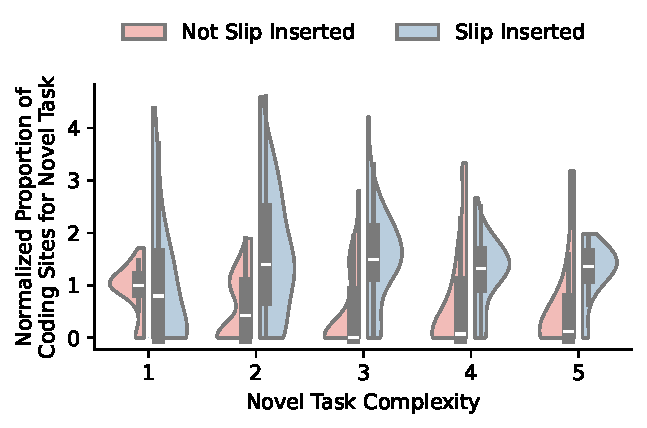
\includegraphics[
width=\linewidth
]{binder/binder/teeplots/density-norm=width+hue=prev-slip-insertion-cumulative-count+kind=violin+viz=catplot+x=components+y=is-task-coding-site+ext=.pdf}
\caption{%
  \textbf{Slip-duplicated sites are overrepresented among \textit{de novo} coding sites for complex traits.}
  \footnotesize
  Distributions compare frequencies of previously slip-duplicated and non-slip-duplicated sites among  \textit{de novo} task coding sites, normalized to neutral expectation.
  Values greater than 1 indicate that sites are overrepresented among the coding sites of novel traits compared to their background frequency.
  Differences between slip-duplicated and non slip-duplicated sites are significant for tasks requiring 2 or more NAND components (Mann-Whitney test; $p < 0.01$).
} \label{fig:potentiation}
\end{figure}
